\section{Testing}

\subsection{Continous Testing}
\begin{frame}
\frametitle{Continuous Testing}

\begin{definition}
Continuous testing uses excess cycles on a developer’s workstation to continuously run regression tests in the background, providing rapid feedback about test failures as code is edited (Saff and Ernst, 2005).
\end{definition}

We use continuous testing and Test-driven Development approach to develop SQAT.

\end{frame}

\subsection{Travis CI and Coverall}
\begin{frame}
\frametitle{Travis CI and Coverall}

\only<1>{
  \begin{center}
  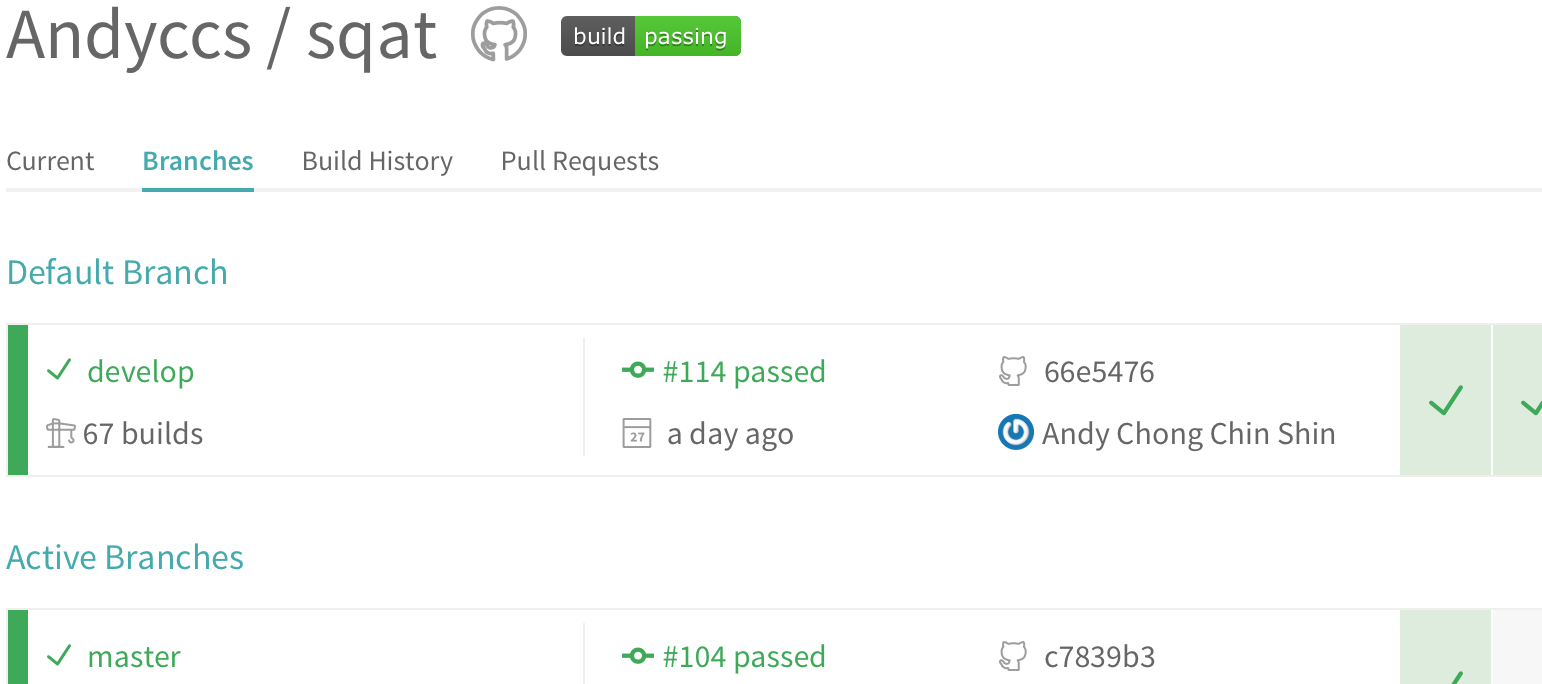
\includegraphics[scale=0.36]{travis_ci}
  \end{center}

  When we check in codes to SQAT code repository, Travis CI will build and test the codes immediately.

  \tiny{\url{Source: https://travis-ci.org/Andyccs/sqat}}
}
\only<2>{
  \begin{center}
  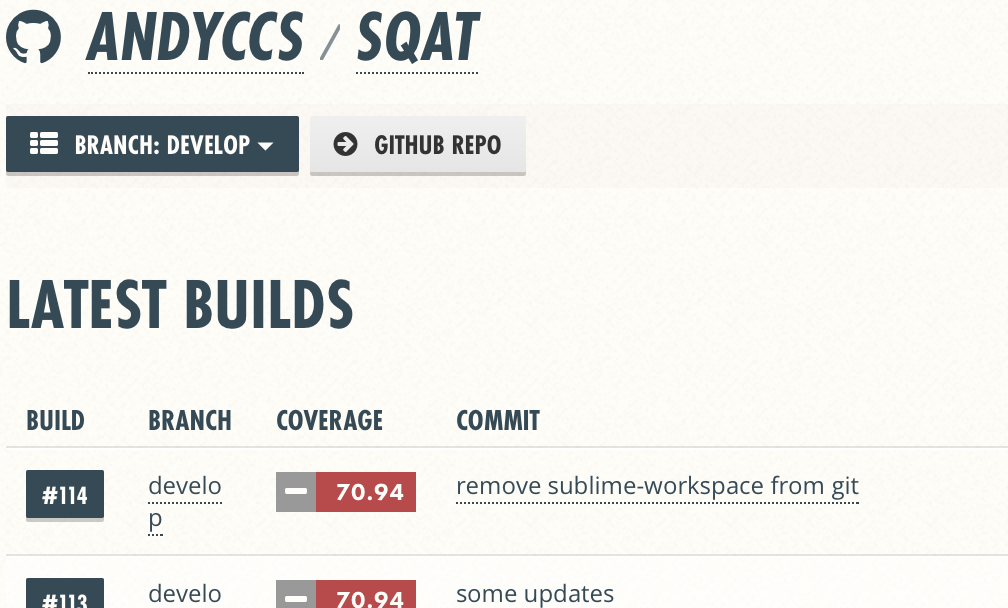
\includegraphics[scale=0.36]{coverall}
  \end{center}

  Similary, Coverall will run all test cases in the repository an generate a code coverage report. 

  \tiny{\url{Source: https://coveralls.io/github/Andyccs/sqat}}
}
\end{frame}